% !TEX root = ../Thesis.tex

% overzicht van alle topics, samengevat waar mogelijk, die nog als todo staan of waar we verdere verbertering voorstellen
\section{Recommendations}
\label{sec:recommendations}
Although we believe the new parser is a large step forward, we also recognize that there are still improvements to be made.

Ampersand is growing and changing in a fast pace.
This is a direct consequence of a project involved with research and active development.
In such projects, it is often impossible to predict which functionalities will be necessary and to design the domain-specific language accordingly beforehand.

As expected we see that most of the remaining issues are related to the grammar ambiguities that force backtracking.
Also the parse tree is not consistently designed.
These issues are mentioned in \autoref{recommendations:design}.
Other improvements are also possible in the test framework delivered, which are mentioned in \autoref{recommendations:tests}.
Finally, we missed more support from the Ampersand website and/or wiki.
This is explained in \autoref{recommendations:website}.

% !TEX root = ../Documentation.tex

\section{Design}
\label{sec:design}
% !TEX root = ../Documentation.tex

\subsection{System overview}
\label{design:system-overview}
  The parser module overview is given in \autoref{fig:ParserModules}.
  \begin{figure}[ht]%
    \centering
    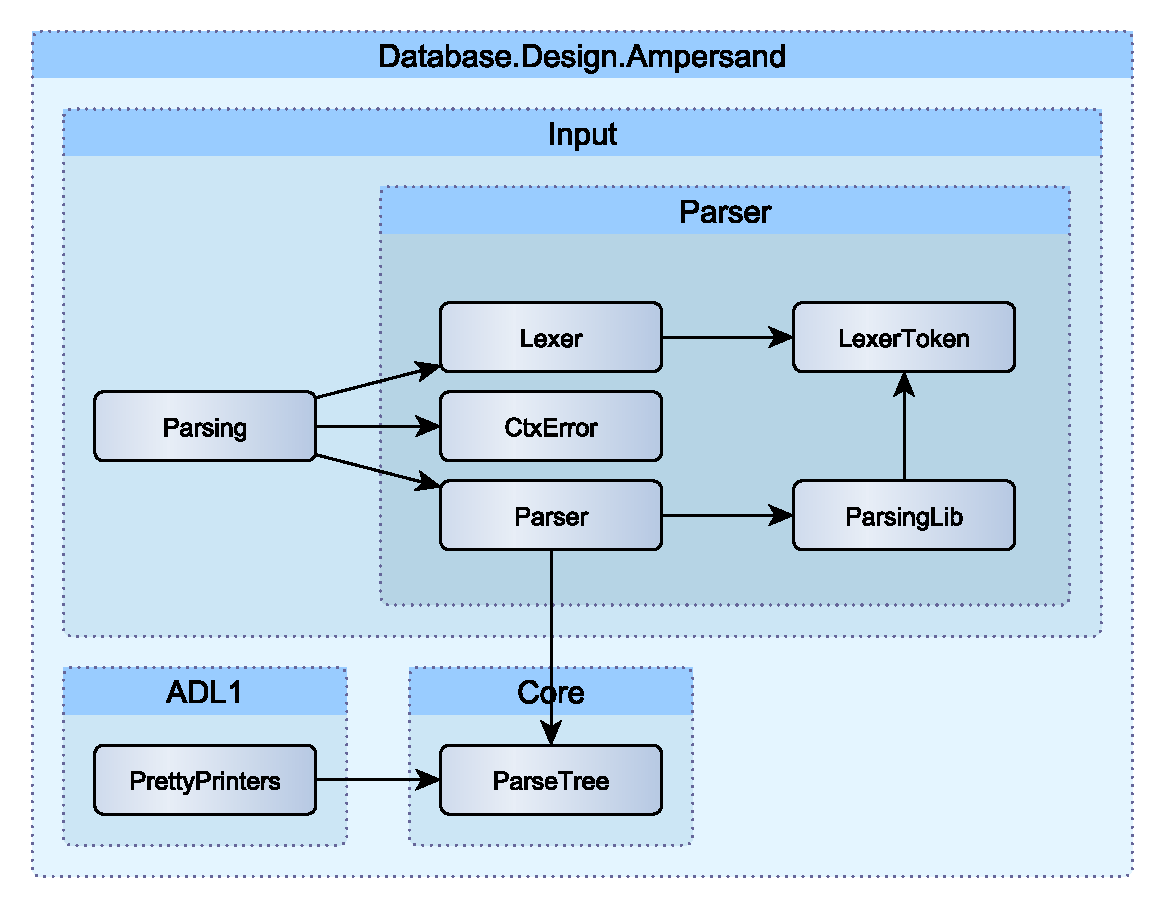
\includegraphics[width=0.7\columnwidth]{Figures/ParserModules}
    \caption{The modules relevant for the parser and their dependencies}
    \label{fig:ParserModules}
  \end{figure}%

  The parsing process starts in the module \code{Parsing}.
  As a first step, the input string is sliced into tokens by the \code{lexer} module.
  Once the input string is separated into the token structure as defined in the module \code{LexerToken} the next step is to actually parse the tokens by the \code{Parser}.
  The parser will use the \code{ParsingLib} to create the parse tree as defined in \code{ParseTree}.

  ~\\\noindent
  Each main module has the following responsibilities:
  %
  \begin{description}
    \item[Parsing] module that implements the interface of the parser with the rest of the system.
      It is responsible for reading the input files, calling the lexer and the parser and returning a parse tree as result (or a parse error).

    \item[Lexer/LexerToken] modules responsible for recognizing the input characters and converting them to tokens.
      The new lexer, together with its sub-modules, splits the input strings into the token structure defined in \code{LexerToken}.
      This list of tokens is the actual input for the parser.

    \item[Parser] module responsible for executing the parsing itself.
      It accepts the tokens that are allowed in each grammar production and generates the corresponding parse tree.
      The parser is described in \autoref{design:new-parser}.
 \end{description}

  \noindent
  Several supporting modules are defined used by one or more main modules:
  \begin{description}
    \item[ParsingLib] library that contains several useful functions to assist the parser, e.g. token recognition.
      These functions are not depending on the specific grammar rules.
      
    \item[ParseTree] external module containing the parse tree data structures.
      Only details of this module have been changed during this project (e.g. field ordering).
    
    \item[PrettyPrinters] contains instances of the \code{Pretty} type class for the parse tree data types and the functions responsible for printing the parse tree to ADL scripts in a `pretty' way.

    \item[CtxError] contains the data structures responsible for the parse errors and their location.
      This module has not been refactored as a part of this project.
    
  \end{description}

% !TEX root = ../Thesis.tex

\subsection{Lexer}
\label{analysis:lexer}
The lexer module is responsible to split up the input stream into tokens.
Tokens are meaningful pieces of the input string that can be recognized by the parser.

The following improvement points were identified after analysis:
\begin{description}
  \item[Dispersed error messages]
    The error messages produced by the lexer are of good quality.
    Each error message is however defined directly within the corresponding lexer function making the maintenance harder.
  \item[Complex token structure]
    The token structure is complex and confusing.
    Two values are present in the token, of which one \texttt{val1} is never used.
    There is no distinction between the values used to identify the content of the token and the ones to determine the position of the token.
  \item[Module structuring]
    In the lexer, the actual lexing functions are intermingled with data types, supporting functions and error message texts.
    This makes the lexer hard to understand and to maintain.
  \item[Language support]
    The errors are returned in English only, no multilingual support is available.
  \item[No support for warnings]
    The lexer can only return errors, warnings are not supported. 
  \item[Strings only]
    Token values are stored as strings for all types, with no conversion of integer values.
  \item[Lacking documentation]
    There was no documentation available on how the lexer was designed and structured.
\end{description}


\subsubsection{Token structure}
The old token has the following structure:

\begin{verbatim}
data Token = Tok { tp' :: TokenType
                 , val1 :: String
                 , val2 :: String
                 , pos :: !Pos
                 , file :: !Filename
                 }

data TokenType
  = TkSymbol
  | TkVarid
  | TkConid
  | TkKeyword
  | TkOp
  | TkString
  | TkExpl
  | TkAtom
  | TkChar
  | TkInteger8
  | TkInteger10
  | TkInteger16
  | TkTextnm
  | TkTextln
  | TkSpace
  | TkError
  deriving (Eq, Ord)
\end{verbatim}
%
The arguments have the following purpose:
\begin{description}
  \item[TokenType]
    Identification of the token type. %, i.e. \texttt{TkSymbol}, \texttt{TkVarid}, \texttt{TkConid}, \texttt{TkKeyword}, \texttt{TkOp}, \texttt{TkString}, \texttt{TkExpl}, \texttt{TkAtom}, \texttt{TkChar}, \texttt{TkInteger8}, \texttt{TkInteger10}, \texttt{TkInteger16}, \texttt{TkTextnm}, \texttt{TkTextln}, \texttt{TkSpace} or \texttt{TkError}.
  \item[val1]
    This string argument is not used in the lexer.
    In the case of a \texttt{keyToken} creation, the value is filled in, but we could not find any purpose for this argument.
  \item[val2]
    The actual token content, stored as a string, including the integer values.
  \item[pos]
    Line and column number.
  \item[file]
     Filename in which the token is located.
\end{description}

% !TEX root = ../Thesis.tex

\subsection{New Parser}
\lipsum[5]
% !TEX root = ../Thesis.tex

\subsection{Parse tree (R-M)}
\label{analysis:parse-tree}
The parse tree (also known as P-structure) is a data structure that very much resembles the EBNF description.
The root of the tree is the \code{P\_Context} structure, and every leaf of the tree has a field for the location where it was found in the ADL code (the \code{Origin} structure).
The tree is consistently defined with the record syntax and is well documented.

However, the constructions are not completely pure, since some transformations are necessary from the ADL to the P-structure.
This forces the parser to do more than only parsing.
Also, the order of the fields can be confusing; sometimes \code{Origin} is the first field and sometimes it is not.

During this project, small changes to the parse tree have been done.
These changes are described in \autoref{design:parse-tree}.

% !TEX root = ../Parsing.tex

\section{User-friendly error messages}
\label{sec:errors}
The most important feature of the parser that will be built, is that it should generate user-friendly error messages.
To understand what kinds of messages can be (and should be) generated, a research will be done on what good errors are and how to generate them.

This is also related to the choice of the parsing library, since the chosen library should support the generation of good errors without extensive effort.
Coincidently, a good source of knowledge are the papers of the supervisor, Bastiaan Heeren, who has done his PhD thesis on the generation of top quality type error messages\cite{heeren-error}.

% !TEX root = ../Documentation.tex

\subsection{Next steps (M)}
\label{subsec:design-next-steps}

During the parser re-implementation and code re-factoring to enhance the code maintainability, we noticed potential improvement topics in Ampersand.
Were possible, with respect to our project requirements and our milestones, we integrated these topics in the new parser.
Some topics we could not handle due to time constraints or given the undesired impact on the surrounding modules.
It would be a pity if these improvement ideas were lost as these can help the Ampersand team to further enhance the tool.
This section summarizes our improvement suggestions, both generic as specific ones, for the Ampersand tool.

\begin{description}
  \item[Syntax improvements]
    In the syntax, we discovered some statements which are not pure LL(k) statements.
    The Parsec \texttt{try} function allows the backtracking in the parser, avoiding that input is consumed which is still needed in another parse statements if the parse function can not succeed successfully.
    Using \texttt{try} we can handle this situation but the backtracking has a negative impact of the parser performance whilst it adds complexity to the parser module. 
    Our suggestion is to further optimize the Ampersand syntax to establish a pure predictive syntax in which no backtracking is needed.
    This will not only improve the parser performance and maintainability, the syntax simplifications will .
    The syntax statements in which backtracking is needed, including the reasons why, are listed in section \autoref{subsec:backtracking}.

  \item[Warnings]
    An improvement point in the new lexer is that warnings are now supported. 
    Warnings are however not yet integrated in the Ampersand tool.
    There is no need to stop the compiling process for warnings, as the reasons behind them can make sense.
    Warnings can, however, support the user identifying the cause of unexpected results, although the compilation could be completed successfully.
    Our suggestion is to add the list of warnings to the design artifacts of Ampersand, available for the user to reflect on is needed.

  \item[Uniform parse tree structure]

todo


  \item[Manual overrule of error message]
    Our analysis of the new error messages showed that the quality of these improved distinctively.
    Parsec provides to possibility to overrule the standard Parsec error message by an own formulated message.
    During our implementation we decided to stick to the standard if the standard error message was, at least, sufficient.
    If the Ampersand teams want to tweak some error message after all, this can be realized using the \texttt{<?>} Parsec function.
    Placing the \texttt{<?>} after the parser, followed by a string, changes the standard Parsec text after the keyword `expecting'.

\end{description}


% !TEX root = ../Thesis.tex

\section{Test Report}
\label{sec:tests}

% !TEX root = ../Thesis.tex

\subsection{Test suite}
  Together with the new parser, a test suite has been developed.
  This test suite has been used to verify the performance and correctness of the new parser.
  The source code can be found in the folder \code{src/Database/Design/Ampersand/Test} within the Ampersand repository.

  The test suite runs in three steps (see \autoref{fig:TestModules}).
  The first step is to check if a list of input files can be parsed successfully. 
  If no issues are found during the parsing, the same list is used by the module \code{RunAmpersand} in which all input scripts are processed completely by Ampersand.
  As a final step, a series of random generated parse tree structures is generated, translated in ADL files and tested.
  Each of the modules are described in the following subsection.
  %
  \begin{figure}[ht]%
    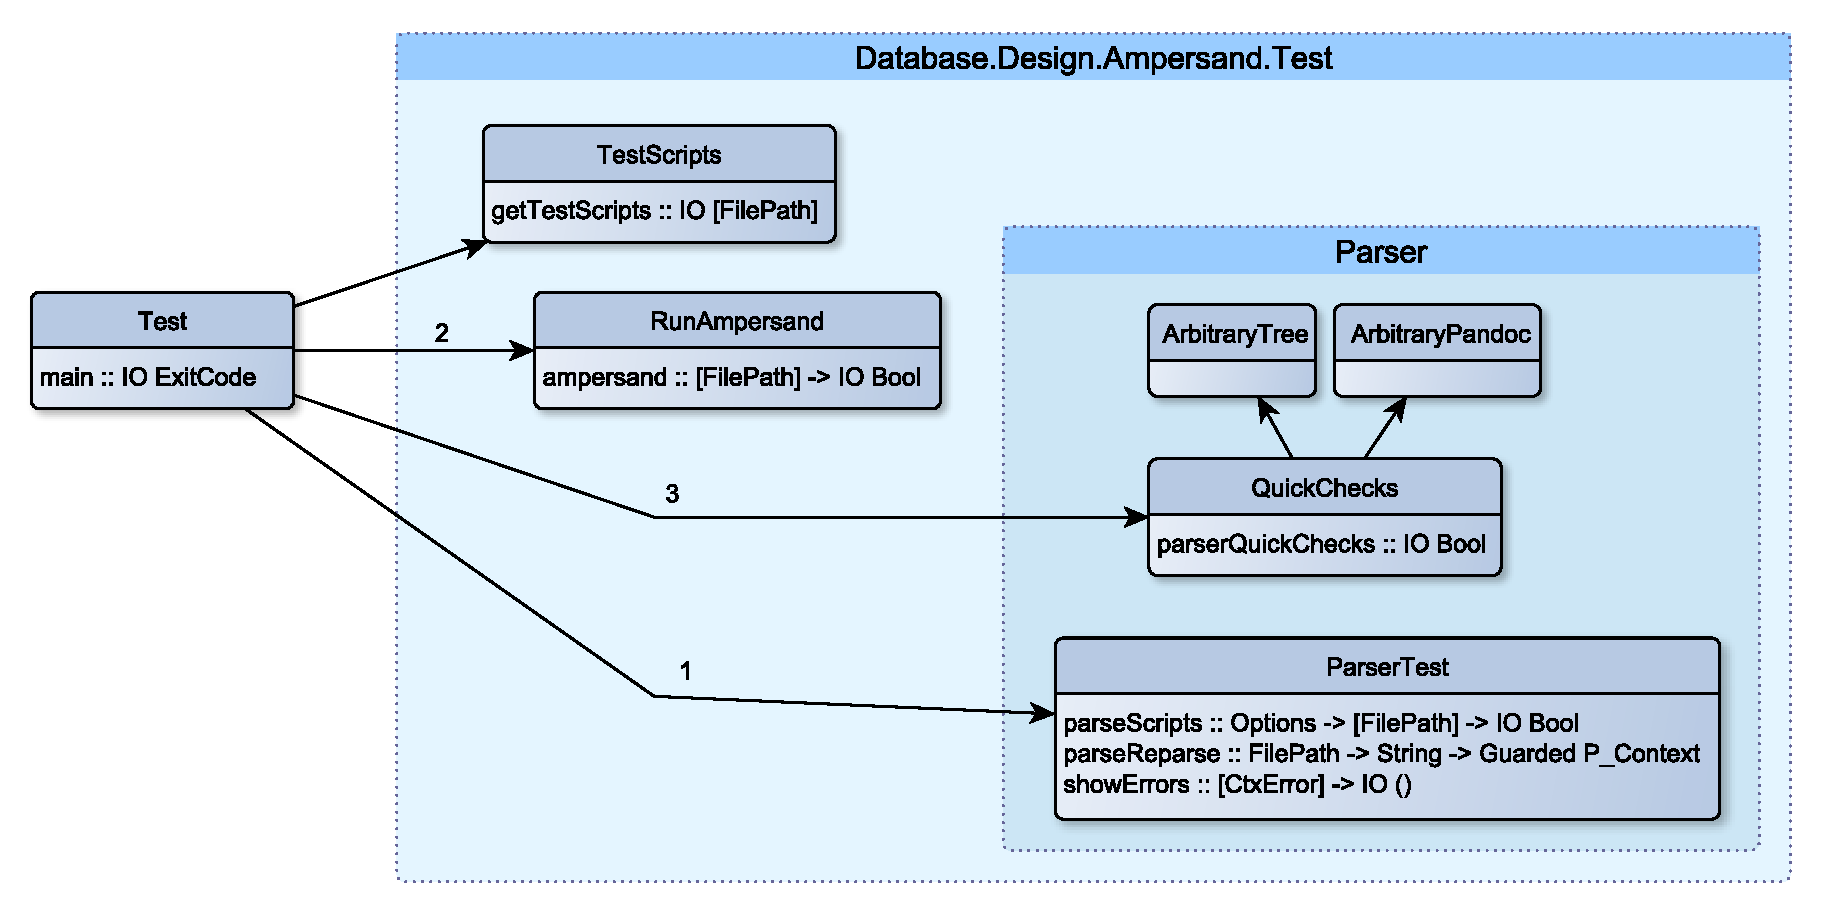
\includegraphics[width=\columnwidth]{Figures/TestModules}
    \caption{Test suite modules with their exported functions}
    \label{fig:TestModules}
  \end{figure}%

  %todo: herwerking op basis van de opmerkingen van Bastiaan
  \subsubsection{Modules}
  \label{tests:test-modules}
  In this section a short description of each module is given:%
  %
  \begin{description}
    \item[Test] contains the \code{main} method that can be executed to run the test suite.
      The \code{main} function calls each of the other modules in sequence, stopping if any of them returns \code{False}.
      When all tests have been successful, the return code is \code{ExitSuccess}.
      Otherwise, the return code is naturally \code{ExitFailure}.
	  
    \item[ParserTest] exports three functions that are the core of testing the parser:
      \begin{itemize}
        \item \code{parseScripts} receives a list of files to parse, and checks that every file can be parsed successfully.
        \item \code{parseReparse} tries to parse a file, and if successful, pretty-prints the result and parses it again.
        \item \code{showErrors} prints the given parse errors to the output.
      \end{itemize}
    
    \item[RunAmpersand] receives a list of files, and checks that every file can be executed successfully by Ampersand.
      This tests thus not only the parser, but also the interface between the parser and the type checker, as the rest of the Ampersand chain.
  \end{description}
	  
  The following modules are supporting one ore more of the three main modules:
  \begin{description}	  
    \item[TestScripts] retrieves a list of scripts that can be used for the different tests.
      It searches for tests within the folder \code{ArchitectureAndDesign}, and contains a list of scripts from the \code{ampersand-models} repository, that can be changed at a later moment if wished.
      Note that all the ADL-scripts listed in this section must be correct for the parser and the type checker.
      During development, the list was limited to the scripts that could be successfully executed by the original Ampersand version.   
	  
    \item[QuickChecks] generates random parse tree structures and generates the corresponding ADL-script by pretty printing the parse tree.
      This ADL-script is then fed back to the parser through the \code{parseReparse} function, to verify that the parser can accept any random input.
      More information on the quick checks is given in subsection~\ref{tests:quick-check}.
    
    \item[ArbitraryTree] is a support module that gives \code{Arbitrary} instances to all parse-tree structures.
      This is used by QuickCheck as described in subsection~\ref{tests:quick-check}.
    
    \item[ArbitraryPandoc] contains \code{Arbitrary} instances to the Pandoc data types.
      This file has not been developed in this project, but copied from the \code{jgm/pandoc} project with the GPL license.
  \end{description}

  \subsubsection{QuickCheck and pretty printing}
  \label{tests:quick-check}
  The most innovative part of the test suite is the use of random structures to test the parser.
  In this section we describe how this generation is implemented.
  
  The main role in the generation of random structures is played by the support library QuickCheck, which has been added to the Ampersand project.
  QuickCheck is able to generate any data structure randomly.
  However, since the parse tree is a custom structure that must obey specific rules, QuickCheck requires the specification of these rules by instances of the \code{Arbitrary} class.
  
  Every data structure in the parse tree has received an \code{Arbitrary} instance used for test purposes.
  The instances can be found in the module \code{Database.Design.Ampersand.Test.Parser\-.ArbitraryTree}, as described in subsection~\ref{tests:test-modules}.
  
  After generating the random parse trees, the test suite needs to convert them to ADL-scripts.
  The conversion of parse tree to source code is also known as pretty printing.
  As the pretty printing is seen as part of the parse tree, it is not included in the Test modules, but is part of the input subsystem.
  The pretty printing instances are found in the module \code{Database.Design.Ampersand.ADL1.PrettyPrinters}.
  This module makes use of the library \code{Text.PrettyPrint.Leijen}, that outlines the output so it is indeed `pretty'.
  
  Now that the ADL source is available, the parser is executed.
  The result of the parser is checked to be equal to the generated tree by the property \code{prop\_pretty}.
  The property is currently tested for 64 generated parse trees in the test suite.
  If the test fails for any generated structure, the test suite fails with an appropriate error.
  
  \subsubsection{Running the tests}
  During the parser development, the \code{main} function of the parser tests has been executed manually, through a batch file.
  This is mainly done because the project team did not have access to the Sentinel server, and no documentation was available on how to run Sentinel locally on a Windows machine.
  However, now that the parser is being delivered, it should be integrated with the other existing Ampersand/Sentinel tests.
  We leave the option open for the Ampersand development team to either add the Sentinel jobs to this test suite, or to add the parser test suite to the Sentinel jobs.
  
  \subsubsection{Test coverage}
  %TODO: Update the numbers when delivery is ready.
  The main objective of the test suite is naturally to test the parser.
  By using HPC (Haskell Program Coverage) we verified that the most important parts of the code were well tested.
  For instance, the \code{Parser} module is covered by 96\%.
  \code{ParsingLib} is 87\% covered, while the module \code{Lexer} is 82\% tested.
  Finally, the module \code{PrettyPrinters} is 98\% covered.
  The complete list with the code coverage is available in the generated HPC report, which is part of the \hyperref[app:docs]{project documentation (appendix)}.
  
  Note that the parts of the code that were not tested, could not be tested for two reasons: only valid ADL files are tested automatically; the incorrect files are tested manually (see \autoref{tests:errors}).
  The other reason is that the ADL files provided did not contain all possible grammar constructions.
  Given the extend to which the errors are tested manually we believe that the full test coverage will be very close to 100\%.
  
% !TEX root = ../Parsing.tex

\section{User-friendly error messages}
\label{sec:errors}
The most important feature of the parser that will be built, is that it should generate user-friendly error messages.
To understand what kinds of messages can be (and should be) generated, a research will be done on what good errors are and how to generate them.

This is also related to the choice of the parsing library, since the chosen library should support the generation of good errors without extensive effort.
Coincidently, a good source of knowledge are the papers of the supervisor, Bastiaan Heeren, who has done his PhD thesis on the generation of top quality type error messages\cite{heeren-error}.

% !TEX root = ../Documentation.tex

\subsection{Website and Wiki (R-D)}
\label{recommendations:website}
During the initiation phase of the project we tried to gather as much information as possible regarding the Ampersand project.
The Ampersand project currently has 2 information sources, a Wiki page and a GitHub page.
The Wiki page focuses on the goals and the practical usage of Ampersand where the GitHub page is more oriented to the Ampersand developers.

We experienced that is was not always easy to find the information we were looking for on these sites.
Some information was outdated or sometimes the link was broken. 
Our suggestion is to have both sites more aligned to each other and to take some time to refresh the current Wiki page.
This will make it easier for new Ampersand users to have a kick-start in the Ampersand world.

